% Generated by Sphinx.
\def\sphinxdocclass{report}
\documentclass[letterpaper,10pt,openany,oneside]{sphinxmanual}
\usepackage[utf8]{inputenc}
\DeclareUnicodeCharacter{00A0}{\nobreakspace}
\usepackage[T1]{fontenc}
\usepackage[english]{babel}
\usepackage{times}
\usepackage[Bjarne]{fncychap}
\usepackage{longtable}
\usepackage{sphinx}
\usepackage{multirow}


\title{Visualize Numerical Integration}
\date{July 21, 2014}
\release{}
\author{CSInParallel Project}
\newcommand{\sphinxlogo}{}
\renewcommand{\releasename}{}
\makeindex

\makeatletter
\def\PYG@reset{\let\PYG@it=\relax \let\PYG@bf=\relax%
    \let\PYG@ul=\relax \let\PYG@tc=\relax%
    \let\PYG@bc=\relax \let\PYG@ff=\relax}
\def\PYG@tok#1{\csname PYG@tok@#1\endcsname}
\def\PYG@toks#1+{\ifx\relax#1\empty\else%
    \PYG@tok{#1}\expandafter\PYG@toks\fi}
\def\PYG@do#1{\PYG@bc{\PYG@tc{\PYG@ul{%
    \PYG@it{\PYG@bf{\PYG@ff{#1}}}}}}}
\def\PYG#1#2{\PYG@reset\PYG@toks#1+\relax+\PYG@do{#2}}

\expandafter\def\csname PYG@tok@gd\endcsname{\def\PYG@tc##1{\textcolor[rgb]{0.63,0.00,0.00}{##1}}}
\expandafter\def\csname PYG@tok@gu\endcsname{\let\PYG@bf=\textbf\def\PYG@tc##1{\textcolor[rgb]{0.50,0.00,0.50}{##1}}}
\expandafter\def\csname PYG@tok@gt\endcsname{\def\PYG@tc##1{\textcolor[rgb]{0.00,0.25,0.82}{##1}}}
\expandafter\def\csname PYG@tok@gs\endcsname{\let\PYG@bf=\textbf}
\expandafter\def\csname PYG@tok@gr\endcsname{\def\PYG@tc##1{\textcolor[rgb]{1.00,0.00,0.00}{##1}}}
\expandafter\def\csname PYG@tok@cm\endcsname{\let\PYG@it=\textit\def\PYG@tc##1{\textcolor[rgb]{0.25,0.50,0.56}{##1}}}
\expandafter\def\csname PYG@tok@vg\endcsname{\def\PYG@tc##1{\textcolor[rgb]{0.73,0.38,0.84}{##1}}}
\expandafter\def\csname PYG@tok@m\endcsname{\def\PYG@tc##1{\textcolor[rgb]{0.13,0.50,0.31}{##1}}}
\expandafter\def\csname PYG@tok@mh\endcsname{\def\PYG@tc##1{\textcolor[rgb]{0.13,0.50,0.31}{##1}}}
\expandafter\def\csname PYG@tok@cs\endcsname{\def\PYG@tc##1{\textcolor[rgb]{0.25,0.50,0.56}{##1}}\def\PYG@bc##1{\setlength{\fboxsep}{0pt}\colorbox[rgb]{1.00,0.94,0.94}{\strut ##1}}}
\expandafter\def\csname PYG@tok@ge\endcsname{\let\PYG@it=\textit}
\expandafter\def\csname PYG@tok@vc\endcsname{\def\PYG@tc##1{\textcolor[rgb]{0.73,0.38,0.84}{##1}}}
\expandafter\def\csname PYG@tok@il\endcsname{\def\PYG@tc##1{\textcolor[rgb]{0.13,0.50,0.31}{##1}}}
\expandafter\def\csname PYG@tok@go\endcsname{\def\PYG@tc##1{\textcolor[rgb]{0.19,0.19,0.19}{##1}}}
\expandafter\def\csname PYG@tok@cp\endcsname{\def\PYG@tc##1{\textcolor[rgb]{0.00,0.44,0.13}{##1}}}
\expandafter\def\csname PYG@tok@gi\endcsname{\def\PYG@tc##1{\textcolor[rgb]{0.00,0.63,0.00}{##1}}}
\expandafter\def\csname PYG@tok@gh\endcsname{\let\PYG@bf=\textbf\def\PYG@tc##1{\textcolor[rgb]{0.00,0.00,0.50}{##1}}}
\expandafter\def\csname PYG@tok@ni\endcsname{\let\PYG@bf=\textbf\def\PYG@tc##1{\textcolor[rgb]{0.84,0.33,0.22}{##1}}}
\expandafter\def\csname PYG@tok@nl\endcsname{\let\PYG@bf=\textbf\def\PYG@tc##1{\textcolor[rgb]{0.00,0.13,0.44}{##1}}}
\expandafter\def\csname PYG@tok@nn\endcsname{\let\PYG@bf=\textbf\def\PYG@tc##1{\textcolor[rgb]{0.05,0.52,0.71}{##1}}}
\expandafter\def\csname PYG@tok@no\endcsname{\def\PYG@tc##1{\textcolor[rgb]{0.38,0.68,0.84}{##1}}}
\expandafter\def\csname PYG@tok@na\endcsname{\def\PYG@tc##1{\textcolor[rgb]{0.25,0.44,0.63}{##1}}}
\expandafter\def\csname PYG@tok@nb\endcsname{\def\PYG@tc##1{\textcolor[rgb]{0.00,0.44,0.13}{##1}}}
\expandafter\def\csname PYG@tok@nc\endcsname{\let\PYG@bf=\textbf\def\PYG@tc##1{\textcolor[rgb]{0.05,0.52,0.71}{##1}}}
\expandafter\def\csname PYG@tok@nd\endcsname{\let\PYG@bf=\textbf\def\PYG@tc##1{\textcolor[rgb]{0.33,0.33,0.33}{##1}}}
\expandafter\def\csname PYG@tok@ne\endcsname{\def\PYG@tc##1{\textcolor[rgb]{0.00,0.44,0.13}{##1}}}
\expandafter\def\csname PYG@tok@nf\endcsname{\def\PYG@tc##1{\textcolor[rgb]{0.02,0.16,0.49}{##1}}}
\expandafter\def\csname PYG@tok@si\endcsname{\let\PYG@it=\textit\def\PYG@tc##1{\textcolor[rgb]{0.44,0.63,0.82}{##1}}}
\expandafter\def\csname PYG@tok@s2\endcsname{\def\PYG@tc##1{\textcolor[rgb]{0.25,0.44,0.63}{##1}}}
\expandafter\def\csname PYG@tok@vi\endcsname{\def\PYG@tc##1{\textcolor[rgb]{0.73,0.38,0.84}{##1}}}
\expandafter\def\csname PYG@tok@nt\endcsname{\let\PYG@bf=\textbf\def\PYG@tc##1{\textcolor[rgb]{0.02,0.16,0.45}{##1}}}
\expandafter\def\csname PYG@tok@nv\endcsname{\def\PYG@tc##1{\textcolor[rgb]{0.73,0.38,0.84}{##1}}}
\expandafter\def\csname PYG@tok@s1\endcsname{\def\PYG@tc##1{\textcolor[rgb]{0.25,0.44,0.63}{##1}}}
\expandafter\def\csname PYG@tok@gp\endcsname{\let\PYG@bf=\textbf\def\PYG@tc##1{\textcolor[rgb]{0.78,0.36,0.04}{##1}}}
\expandafter\def\csname PYG@tok@sh\endcsname{\def\PYG@tc##1{\textcolor[rgb]{0.25,0.44,0.63}{##1}}}
\expandafter\def\csname PYG@tok@ow\endcsname{\let\PYG@bf=\textbf\def\PYG@tc##1{\textcolor[rgb]{0.00,0.44,0.13}{##1}}}
\expandafter\def\csname PYG@tok@sx\endcsname{\def\PYG@tc##1{\textcolor[rgb]{0.78,0.36,0.04}{##1}}}
\expandafter\def\csname PYG@tok@bp\endcsname{\def\PYG@tc##1{\textcolor[rgb]{0.00,0.44,0.13}{##1}}}
\expandafter\def\csname PYG@tok@c1\endcsname{\let\PYG@it=\textit\def\PYG@tc##1{\textcolor[rgb]{0.25,0.50,0.56}{##1}}}
\expandafter\def\csname PYG@tok@kc\endcsname{\let\PYG@bf=\textbf\def\PYG@tc##1{\textcolor[rgb]{0.00,0.44,0.13}{##1}}}
\expandafter\def\csname PYG@tok@c\endcsname{\let\PYG@it=\textit\def\PYG@tc##1{\textcolor[rgb]{0.25,0.50,0.56}{##1}}}
\expandafter\def\csname PYG@tok@mf\endcsname{\def\PYG@tc##1{\textcolor[rgb]{0.13,0.50,0.31}{##1}}}
\expandafter\def\csname PYG@tok@err\endcsname{\def\PYG@bc##1{\setlength{\fboxsep}{0pt}\fcolorbox[rgb]{1.00,0.00,0.00}{1,1,1}{\strut ##1}}}
\expandafter\def\csname PYG@tok@kd\endcsname{\let\PYG@bf=\textbf\def\PYG@tc##1{\textcolor[rgb]{0.00,0.44,0.13}{##1}}}
\expandafter\def\csname PYG@tok@ss\endcsname{\def\PYG@tc##1{\textcolor[rgb]{0.32,0.47,0.09}{##1}}}
\expandafter\def\csname PYG@tok@sr\endcsname{\def\PYG@tc##1{\textcolor[rgb]{0.14,0.33,0.53}{##1}}}
\expandafter\def\csname PYG@tok@mo\endcsname{\def\PYG@tc##1{\textcolor[rgb]{0.13,0.50,0.31}{##1}}}
\expandafter\def\csname PYG@tok@mi\endcsname{\def\PYG@tc##1{\textcolor[rgb]{0.13,0.50,0.31}{##1}}}
\expandafter\def\csname PYG@tok@kn\endcsname{\let\PYG@bf=\textbf\def\PYG@tc##1{\textcolor[rgb]{0.00,0.44,0.13}{##1}}}
\expandafter\def\csname PYG@tok@o\endcsname{\def\PYG@tc##1{\textcolor[rgb]{0.40,0.40,0.40}{##1}}}
\expandafter\def\csname PYG@tok@kr\endcsname{\let\PYG@bf=\textbf\def\PYG@tc##1{\textcolor[rgb]{0.00,0.44,0.13}{##1}}}
\expandafter\def\csname PYG@tok@s\endcsname{\def\PYG@tc##1{\textcolor[rgb]{0.25,0.44,0.63}{##1}}}
\expandafter\def\csname PYG@tok@kp\endcsname{\def\PYG@tc##1{\textcolor[rgb]{0.00,0.44,0.13}{##1}}}
\expandafter\def\csname PYG@tok@w\endcsname{\def\PYG@tc##1{\textcolor[rgb]{0.73,0.73,0.73}{##1}}}
\expandafter\def\csname PYG@tok@kt\endcsname{\def\PYG@tc##1{\textcolor[rgb]{0.56,0.13,0.00}{##1}}}
\expandafter\def\csname PYG@tok@sc\endcsname{\def\PYG@tc##1{\textcolor[rgb]{0.25,0.44,0.63}{##1}}}
\expandafter\def\csname PYG@tok@sb\endcsname{\def\PYG@tc##1{\textcolor[rgb]{0.25,0.44,0.63}{##1}}}
\expandafter\def\csname PYG@tok@k\endcsname{\let\PYG@bf=\textbf\def\PYG@tc##1{\textcolor[rgb]{0.00,0.44,0.13}{##1}}}
\expandafter\def\csname PYG@tok@se\endcsname{\let\PYG@bf=\textbf\def\PYG@tc##1{\textcolor[rgb]{0.25,0.44,0.63}{##1}}}
\expandafter\def\csname PYG@tok@sd\endcsname{\let\PYG@it=\textit\def\PYG@tc##1{\textcolor[rgb]{0.25,0.44,0.63}{##1}}}

\def\PYGZbs{\char`\\}
\def\PYGZus{\char`\_}
\def\PYGZob{\char`\{}
\def\PYGZcb{\char`\}}
\def\PYGZca{\char`\^}
\def\PYGZam{\char`\&}
\def\PYGZlt{\char`\<}
\def\PYGZgt{\char`\>}
\def\PYGZsh{\char`\#}
\def\PYGZpc{\char`\%}
\def\PYGZdl{\char`\$}
\def\PYGZti{\char`\~}
% for compatibility with earlier versions
\def\PYGZat{@}
\def\PYGZlb{[}
\def\PYGZrb{]}
\makeatother

\begin{document}

\maketitle
\tableofcontents
\phantomsection\label{index::doc}


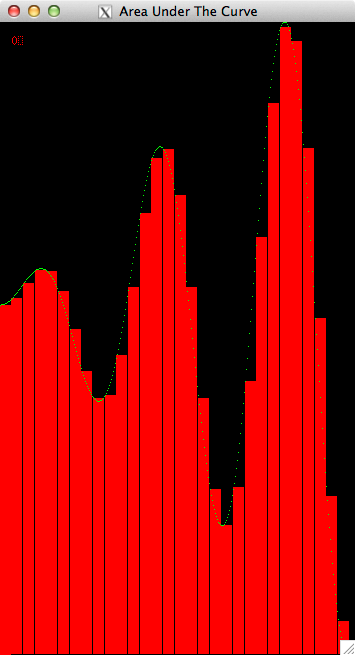
\includegraphics{serial_30rect.png}

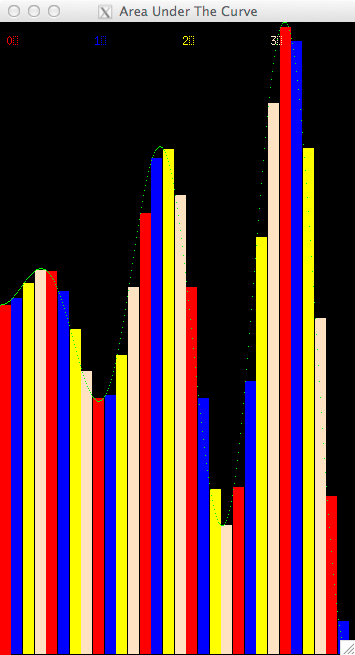
\includegraphics{omp_1chunk_static_30rect.png}

\textbf{Prologue}

This is an activity that steps you through some code we have prepared to help you see how several parallel implementations that solve the numerical integration problem might split the work among processing units.

\textbf{Prerequisites}
\begin{itemize}
\item {} 
Reading the CSinParallel material entitled \emph{Concept: The Data Decomposition Pattern} will provide useful background information regarding the parallel pattern illustrated with these visualizations.

\item {} \begin{description}
\item[{You will need to be able to run these programs on a unix machine with X11 installed and with at least one of the following:}] \leavevmode\begin{itemize}
\item {} 
MPI installed on a single computer or cluster (either MPICH2 or OpenMPI)

\item {} 
gcc with OpenMP (most versions of gcc have this enabled already) and a multicore computer

\end{itemize}

\end{description}

\item {} 
Some knowledge of building C programs using make may be useful.

\item {} 
Some understanding of numerical integration: approximating the integral as the area under a curve with left and right boundaries using the `rectangle rule'.

\end{itemize}

\textbf{Nomenclature}

A \textbf{Processing Unit} is an element of software that can execute instructions on hardware.  On a multicore computer, this would be a \emph{thread} running on a core of the multicore chip.  On a cluster of computers, this would be a \emph{process} running on one of the computers. On a co-processor such as a Graphics Processing Unit (GPU), this would be a \emph{thread} running on one of its many cores.

A program that uses only one processing unit is referred to as a \emph{serial} or \emph{sequential} solution. You are likely most familiar with these types of programs.

\textbf{Code You will Need}

You should download \code{VisArea.tgz} to obtain the code that you will run for the examples shown in the following sections of this reading.


\chapter{The Numerical Integration Problem}
\label{NumericalIntegration::doc}\label{NumericalIntegration:visualize-data-decomposition-of-numerical-integration}\label{NumericalIntegration:the-numerical-integration-problem}
A famous mathematical problem that is easy to compute is to approximate the numerical value of a definite integral of a function from a to b as the area under the curve of that function using the \href{http://en.wikipedia.org/wiki/Rectangle\_method}{rectangle method}.

Given a function, we can approximate its definite integral over the interval (a, b) by adding the values of the areas of contiguous small rectangles whose heights are the value of the function along the interval. Zoomed in on a small portion of a curve for a function, these rectangles look like this:

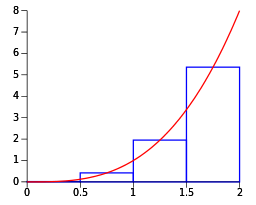
\includegraphics{MidRiemann2.png}

This image is courtesy of Qref on \href{http://commons.wikimedia.org/wiki/File:MidRiemann2.svg}{Wikimedia commons}.


\section{Programming Numerical Integration}
\label{NumericalIntegration:programming-numerical-integration}
Programs written for solving this problem on a given function are fairly straightforward and involve determining the number of rectangles desired over a given interval and computing the value of the function for each rectangle, adding it to an overall sum for the value of the integral.

For a sequential implementation of such a program, the run time is on the order of the number of rectangles. To obtain an accurate result, a large number of rectangles should be used.

The sample code we provide in \code{area.tgz} contains a program that will enable you to visualize several ways that we can make numerical integration run faster by splitting the work of computing the area of each of the rectangles across multiple processing units.  In these examples, we illustrate the types of \emph{data decomposition patterns} that can be used.  In this problem, the data to be computed is the area of each rectangle and we can think of those rectangles as lining up linearly along the x axis as shown above. In the following sections we will walk you through the execution of this code for several different data decompositions of this linear collection of rectangles, using a simple function.

The code you will use is not necessarily meant for you to examine, but instead to run with different hardware and software combinations and see how the decomposition took place.  We built the code to execute in real time, saving the results of which processing unit computed which rectangle. We then graphically display the results by replaying the computations, drawing the rectangles with a time delay so you can visualize what happened.

Continue to the next chapter to begin your journey!


\chapter{The Code, Platforms, and Executing a Serial Version}
\label{Code_Serial::doc}\label{Code_Serial:the-code-platforms-and-executing-a-serial-version}

\section{Parallel Computing Platforms}
\label{Code_Serial:parallel-computing-platforms}
The code we provide will compile and run with the following combinations of platforms. Any computer you use will need linux or unix with X11 (this is how we coded the visualizations).  We have examples that use OpenMP alone, MPI alone, and a combination of MPI and OpenMP (sometimes called hybrid solutions).

The OpenMP examples will run on:
\begin{itemize}
\item {} 
A single multicore machine with an OpenMP-compatible C compiler

\end{itemize}

The MPI examples will run on:
\begin{itemize}
\item {} 
A single multicore computer \emph{or} a cluster with MPICH installed and MPE installed (MPE is a visualization library for MPI based on X11 that comes with MPICH).

\item {} 
A single multicore computer \emph{or} a cluster with OpenMPI installed and MPE installed (with OpenMPI, you need to install MPE separately).

\end{itemize}

The MPI + OpenMP examples will require a single computer or a cluster with MPI, MPE, and an OpenMP compiler all installed.


\section{The Code and Scripts}
\label{Code_Serial:the-code-and-scripts}
You will need to set up the code. First get and uncompress the \code{VisArea.tgz} file like so (these are linux commands):

\begin{Verbatim}[commandchars=\\\{\}]
tar -zxvf VisArea.tgz
ls -R -1
\end{Verbatim}

You should get some output like this:

\begin{Verbatim}[commandchars=\\\{\}]
.:
area
Makefile

./area:
area.c
area.c-mpi
area.h
colors.h
makeExecutable
Makefile
MPEarea.h
MPEcolors.h
Readme
run\PYGZus{}mpi\PYGZus{}chunksOfOne
run\PYGZus{}mpi\PYGZus{}chunksOfOne\PYGZus{}openmp\PYGZus{}equalChunks
run\PYGZus{}mpi\PYGZus{}equalChunks
run\PYGZus{}mpi-openmp\PYGZus{}chunksOfOneDynamic
run\PYGZus{}mpi-openmp\PYGZus{}chunksOfOneStatic
run\PYGZus{}mpi-openmp\PYGZus{}equalChunks
run\PYGZus{}openmp\PYGZus{}chunksOfOneDynamic
run\PYGZus{}openmp\PYGZus{}chunksOfOneStatic
run\PYGZus{}openmp\PYGZus{}equalChunks
run\PYGZus{}serial
structs.h
Xarea.h
\end{Verbatim}

Note that there is a directory called \textbf{area} with its own Makefile and a global Makefile.  You will work inside the directory called \textbf{area}.  From there, we have set up shell scripts to compile and run various types of data decomposition with different hardware and software compinations. Each of these scripts begins with the prefix \emph{run\_}.


\section{Notes about building on your installation}
\label{Code_Serial:notes-about-building-on-your-installation}
You might need to change the path to your X libraries. The place to do that is to edit the LDFLAGS in the the global Makefile (the one outside of the source code folder called \emph{area}).  You can try the first script shown below to test whether this will be a problem for you.


\section{Building and Executing the Serial Version}
\label{Code_Serial:building-and-executing-the-serial-version}
You will need to be logged directly into the computer with the code, MPI, OpenMP, and X11 installed in order to see the X11 visualization that the code produces.  You can also have an X11 client installed on a remote machine in which you use {\color{red}\bfseries{}{}`{}`}ssh -X  {}`{}` to remotely log in to the server with the parallel software and this code installed.

Let's start by trying an example that runs serially, or sequentially, without any parallelization. The script for this is called \code{run\_serial}. You can compile the code and run it like this.

\begin{Verbatim}[commandchars=\\\{\}]
\PYG{n+nb}{cd }area
./run\PYGZus{}serial
\end{Verbatim}

We will run all the rest of the example scripts from the \textbf{area} directory.

An X window displaying how the code executes the computation of the area of each rectangle should appear.  When it completes, it should look like this:

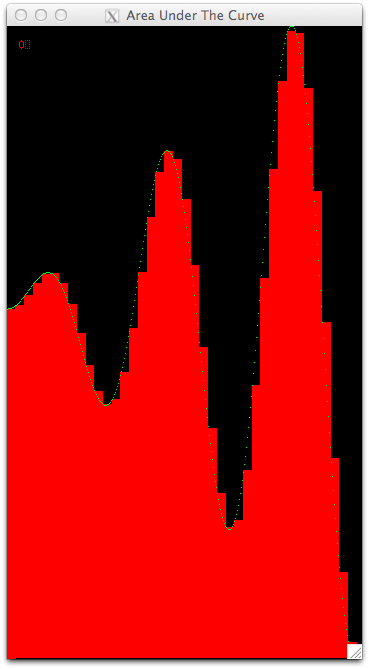
\includegraphics{run_serial.png}

The default curve we use is shown (see below for some more options). Each rectangle is drawn with a single color because one processing unit computed each rectangle, one after another.  In other examples, colors will be used to show which processing unit computed which rectangle.

To close the window, you can type the `q' key if the focus is still in the window. Otherwise, place focus back in the terminal window where you ran the script and type control-c.

We chose some default settings, which you can change to see what happens. For all scripts, you can use the \code{-?} option as follows to see what your options are:

\begin{Verbatim}[commandchars=\\\{\}]
./run\PYGZus{}serial -?
\end{Verbatim}

You should get some output like this:

\begin{Verbatim}[commandchars=\\\{\}]
./run\PYGZus{}serial: illegal option -- ?
usage: ./run\PYGZus{}serial options

This script runs the visualization of computing the area under the curve serially.

OPTIONS:
-t  Throttle \PYG{n+nb}{time }in microseconds
-n  Number of rectangles
-f  Function kind \PYG{o}{(}1, 2 or 3, default \PYG{k}{if }not specified\PYG{o}{)}
-r  Righthand boundary of the curve
\end{Verbatim}

The throttle time will change how quickly the rectangles will be displayed.  These visualizations are designed to be `played' so that you can see what assignments were made.  You can change this time to help you see what is happening.

You can change the number of rectangles under the curve.  Making this smaller or larger might help you envision what is happening in each of the situations we describe in the next few sections. For eaxmple, if you try this:

\begin{Verbatim}[commandchars=\\\{\}]
./run\PYGZus{}serial -n 12
\end{Verbatim}

You can see how this small amount of rectangles does not approximate this curve very well.

However, if you use too many rectangles, it is very hard to see each one. Really high numbers of rectangles will mean that it takes less than one pixel to draw them; this is a situation you want to avoid. About 60 or so is likely the most you should opt for with \code{-n}.

The \code{-f} option will let you pick other curves to display.
\begin{itemize}
\item {} 
Option \emph{1}  is the straight-line function $f(x) = x$.

\item {} 
Option \emph{2} is the positive quarter circle, $f(x) = +\sqrt{r^{2}-x^2}, 0 \le x \le r$

\item {} 
Option \emph{3} is half the period of the sine function, $f(x) = \sin(x), 0 \le x \le \pi$

\item {} 
Option \emph{4}, the default in these example scripts, is the curve $f(x) = x\sin(0.05x)$

\end{itemize}

The \code{-r} option can only be changed with the \code{-f} option \emph{1} or \emph{4}. With \code{-f 1}, values between 400 and 1000 make the most sense to use for \code{-r} (any larger and the window gets too large; any smaller and the window is too small and hard to see.) With \code{-f 4}, the default shown in these scripts is 350 for the right-hand value of x in the function. We recommend going now higher than 600 or so, unless you have a really large monitor.

Now that you know the options, let's you on and try parallel versions of this code.


\chapter{Parallel Displays of the Area Under the Curve}
\label{ParallelVis::doc}\label{ParallelVis:parallel-displays-of-the-area-under-the-curve}
Here we will run the code for various types of data decomposition patterns using OpenMP, MPI, or a combination of MPI and OpenMP.


\section{OpenMP Versions: Shared Memory multicore with threads}
\label{ParallelVis:openmp-versions-shared-memory-multicore-with-threads}
In code that uses OpenMP, the processing unit executing the computation of the area of each rectangle is a \emph{thread} executing on a core of a shred-memory multicore computer.  Let's try a few examples of how OpenMP can map threads to rectangles to be computed.  We consider these rectangles to be computed from left to right, forming a linear set of data values to be computed.

In these visualizations, we run the code in real time as it would get run in openMP, keeping information about which thread computed which rectangle.  The program then displays back which thread computed each rectangle by playing back the recorded information and coloring the rectangles with different color for each thread.


\subsection{Equal chunks of rectangles}
\label{ParallelVis:equal-chunks-of-rectangles}
Try running this script like this on the command line, in the \textbf{area} directory:

\begin{Verbatim}[commandchars=\\\{\}]
./run\PYGZus{}openmp\PYGZus{}equalChunks
\end{Verbatim}

You should see that four threads each computed consecutive equal-sized chunks of rectangles (we sometimes also call this division of work the `blocks' decomposition).  This is a well-used pattern of how to split the work, or decompose the problem, among the threads.  This same pattern is also used frequently in distributed, message passing situations.

\begin{notice}{note}{Note:}
Though the playback in these visualizations may appear to be serial, the threads did run concurrently. We unfortunately have no way of displaying rectangles on the screen in parallel!
\end{notice}


\subsection{Chunks of one, statically assigned}
\label{ParallelVis:chunks-of-one-statically-assigned}
Rather than equal chunks where the size of a chunk that a thread works on is $n/p$, where $p$ is the number of threads and $n$ is the number of rectangles, another possible distribution of work is to have each thread compute one rectangle of the first $p$ rectangles, then go on a compute one of the next group of $p$ rectangles, and so on. If the thread to rectangle assignment is done statically ahead of time, it would look like the results of running this script:

\begin{Verbatim}[commandchars=\\\{\}]
./run\PYGZus{}openmp\PYGZus{}chunksOfOneStatic
\end{Verbatim}

It should look like this when it completes:

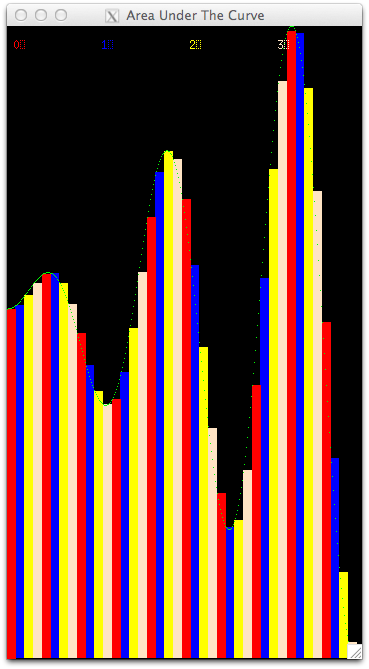
\includegraphics{run_openmp_equalChunks.png}

Note the legend at the top of the window tells you the color for each thread, which are numbered from 0 through 3 for this case. Study this to be certain you understand the assignment of threads to rectangles.

OpenMP can decide for itself which threads will work on which computational elements. This is know as dynamic scheduling.  Try this script for that and see what you observe.  This could be different on different machines and could change each time you run it.

\begin{Verbatim}[commandchars=\\\{\}]
./run\PYGZus{}openmp\PYGZus{}chunksOfOneDynamic
\end{Verbatim}


\section{MPI Examples: distributed message passing}
\label{ParallelVis:mpi-examples-distributed-message-passing}
In MPI, the processing units that run in parallel are \emph{processes}, which are either running on the same machine or more likely across a cluster of machines, where each machine starts its own process.


\subsection{Equal chunks of rectangles}
\label{ParallelVis:id1}
In the case of a cluster of machines, there is one data decomposition pattern that makes the most sense, and that is to partition the work into equal chunks.  Try this script to visualize that case:

\begin{Verbatim}[commandchars=\\\{\}]
./run\PYGZus{}mpi\PYGZus{}equalChunks
\end{Verbatim}

You should see multiple windows displayed, one for each process, with rectangles assigned and computed in the order that they appear inside the function. It should look like this:

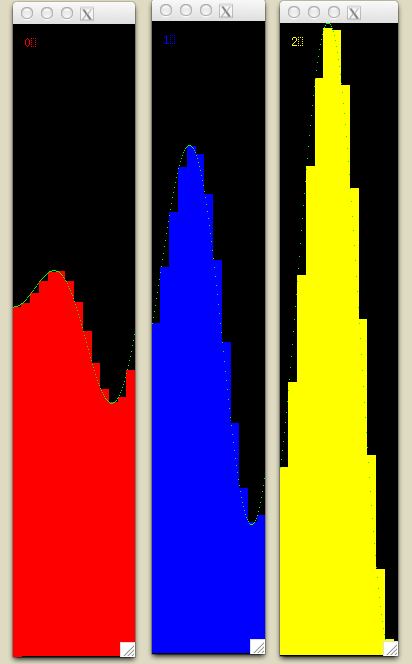
\includegraphics{run_mp_equalChunks.png}


\subsection{Chunks of one, statically assigned}
\label{ParallelVis:id2}
Another possible assignment, especially for a single machine running MPI processes, is to have the processes compute one rectangle each, similar to the single chunk case for OpenMP. Run this and you will see it looks the same as the mapping for OpenMP:

\begin{Verbatim}[commandchars=\\\{\}]
./run\PYGZus{}mpi\PYGZus{}chunksOfOne
\end{Verbatim}


\section{Hybrid: MPI plus OpenMP}
\label{ParallelVis:hybrid-mpi-plus-openmp}
When using MPI across a cluster of machines, if those machines have multicore processors, then each of them can execute code using OpenMP.  The following example script runs this case, where each MPI process gets an equal chunk of the original rectangles, and those chunks are further divided by OpenMP threads.

\begin{Verbatim}[commandchars=\\\{\}]
./run\PYGZus{}mpi-openmp\PYGZus{}equalChunks
\end{Verbatim}

The result for this decomposition looks like this:

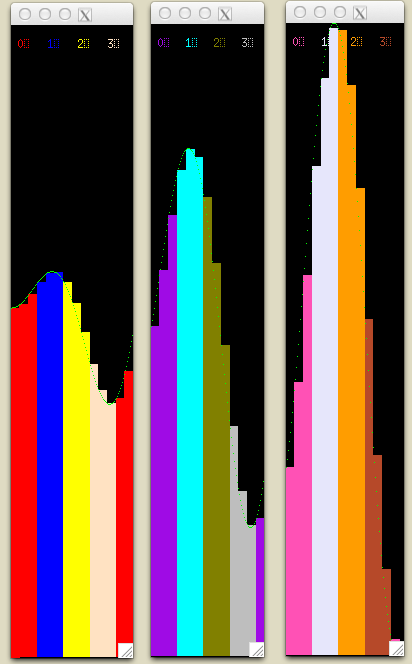
\includegraphics{run_mpi-openmp_equalChunks.png}

There are other possible hybrid combinations- please experiment with some of the other scripts beginning with \code{run\_} that we haven't mentioned here yet to see if you can determine these more complicated patterns.



\renewcommand{\indexname}{Index}
\printindex
\end{document}
